\chapter{Thema}
Die Webanwendung YouStudy bietet eine zentrale Informationsanlaufstelle für Studenten der TH Köln am Campus Gummersbach. Die Website bietet ständig aktuelle Mitteilungen für Studierende, z.B. Informationen welche im Normalfall über das schwarze Brett publiziert werden. Des Weiteren gibt es eine Übersicht über aktuelle Filme des Campus Kino und ihre Termine. Als weiteren Inhalt liefert YouStudy eine Übersicht über die jeweils aktuelle Parkplatzsituation am Campus Gummersbach, sowie den aktuellen Speiseplan der Mensa.


\begin{figure}[ht]
\chapter{Mock Ups}
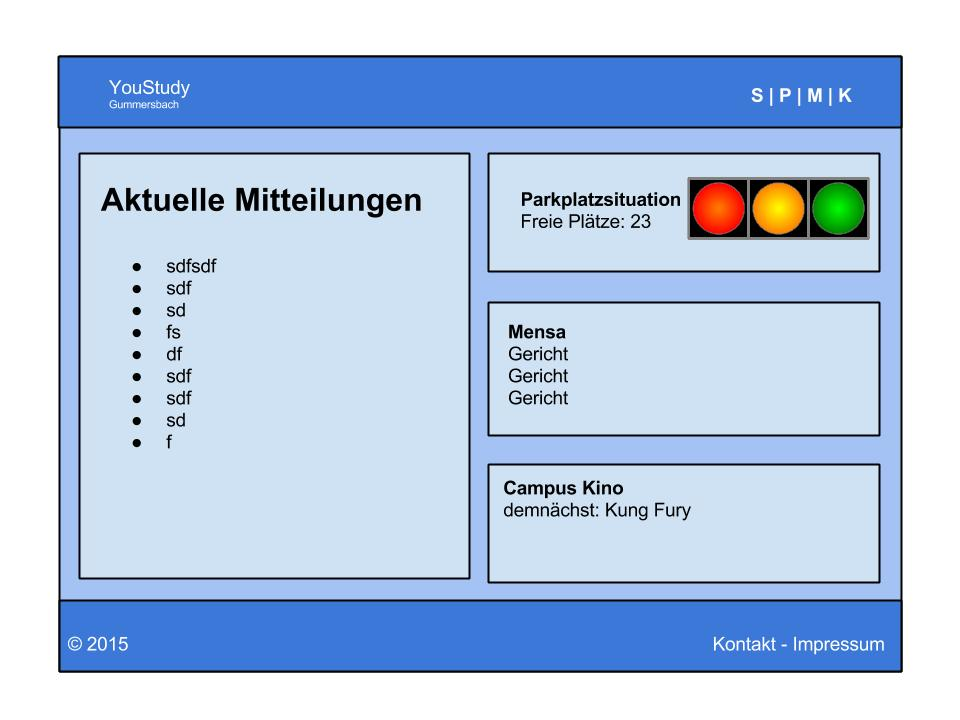
\includegraphics[width=0.9\textwidth]{./img/Startseite}\caption{Startseite Mock Up}\label{fig1}
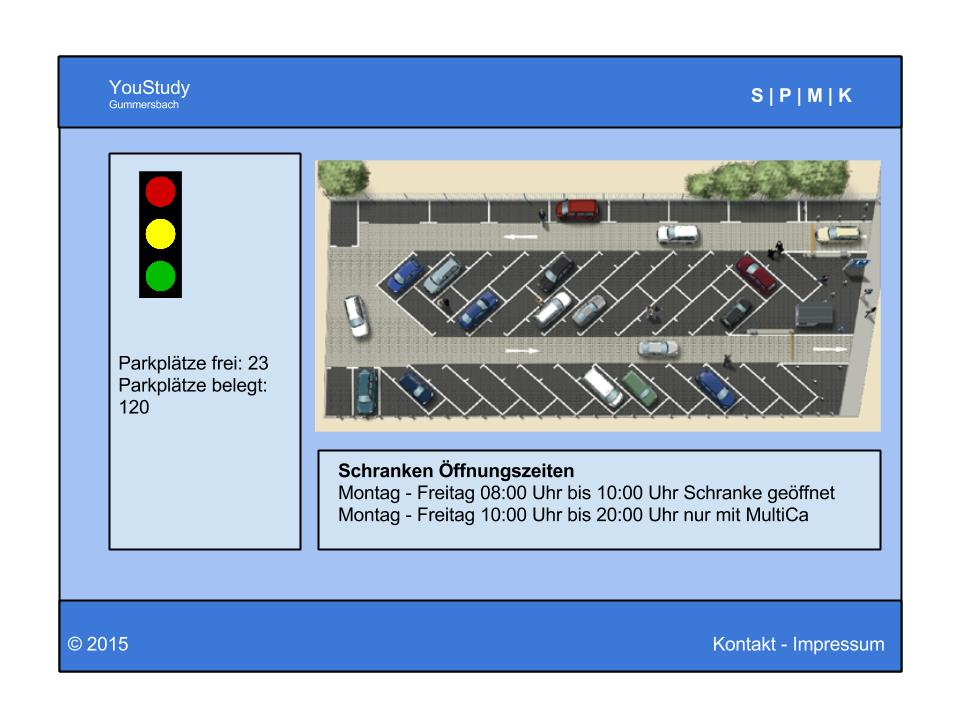
\includegraphics[width=0.9\textwidth]{./img/Parkplatz}\caption{Parkplatz Mock Up}\label{fig2}
\end{figure}

\begin{figure}[ht]
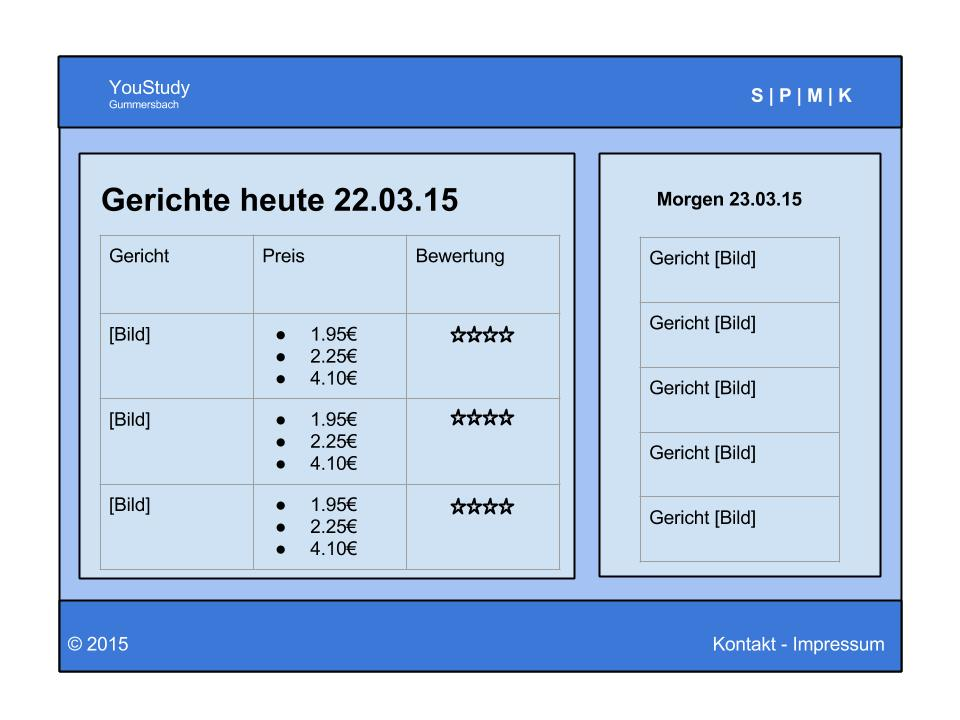
\includegraphics[width=0.9\textwidth]{./img/Mensa}\caption{Mensa Mock Up}\label{fig3}
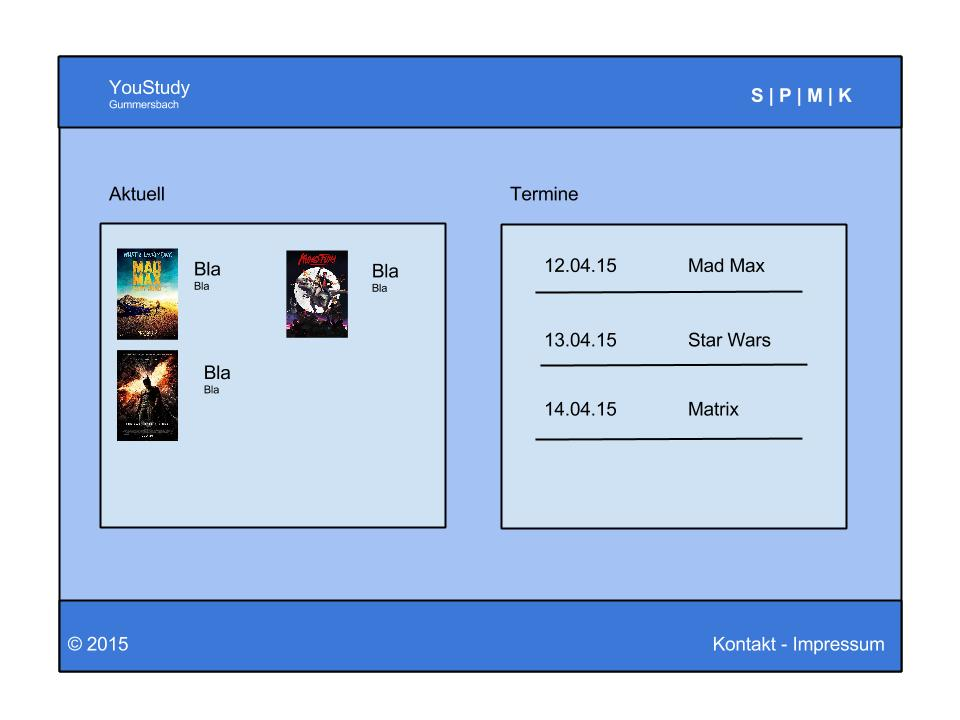
\includegraphics[width=0.9\textwidth]{./img/Kino}\caption{Kino Mock Up}\label{fig4}
\end{figure}
 
\chapter{Datenbankschema}
Im Folgenden sind die zur Anwendung gehörenden Entitäten und Daten zu sehen:
%
% Struktur: movies
%
 \begin{longtable}{|l|c|c|c|l|} 
 \caption{Struktur der Tabelle movies} \label{tab:movies-structure} \\
 \hline \multicolumn{1}{|c|}{\textbf{Spalte}} & \multicolumn{1}{|c|}{\textbf{Typ}} & \multicolumn{1}{|c|}{\textbf{Null}} & \multicolumn{1}{|c|}{\textbf{Standard}} & \multicolumn{1}{|c|}{\textbf{Kommentare}} \\ \hline \hline
\endfirsthead
 \caption{Struktur der Tabelle movies (Fortsetzung)} \\ 
 \hline \multicolumn{1}{|c|}{\textbf{Spalte}} & \multicolumn{1}{|c|}{\textbf{Typ}} & \multicolumn{1}{|c|}{\textbf{Null}} & \multicolumn{1}{|c|}{\textbf{Standard}} & \multicolumn{1}{|c|}{\textbf{Kommentare}} \\ \hline \hline \endhead \endfoot 
\textbf{\textit{id}} & int(11) & Nein & & \\ \hline 
filename & varchar(150) & Nein & & \\ \hline 
poster & mediumblob & Nein & & \\ \hline 
 \end{longtable}

%
% Struktur: users
%
 \begin{longtable}{|l|c|c|c|l|} 
 \caption{Struktur der Tabelle users} \label{tab:users-structure} \\
 \hline \multicolumn{1}{|c|}{\textbf{Spalte}} & \multicolumn{1}{|c|}{\textbf{Typ}} & \multicolumn{1}{|c|}{\textbf{Null}} & \multicolumn{1}{|c|}{\textbf{Standard}} & \multicolumn{1}{|c|}{\textbf{Kommentare}} \\ \hline \hline
\endfirsthead
 \caption{Struktur der Tabelle users (Fortsetzung)} \\ 
 \hline \multicolumn{1}{|c|}{\textbf{Spalte}} & \multicolumn{1}{|c|}{\textbf{Typ}} & \multicolumn{1}{|c|}{\textbf{Null}} & \multicolumn{1}{|c|}{\textbf{Standard}} & \multicolumn{1}{|c|}{\textbf{Kommentare}} \\ \hline \hline \endhead \endfoot 
\textbf{\textit{id}} & int(11) & Nein & & \\ \hline 
username & varchar(50) & Nein & & \\ \hline 
password & varchar(150) & Nein & & \\ \hline 
 \end{longtable}

%
% Struktur: zuo_movie_rating
%
 \begin{longtable}{|l|c|c|c|l|} 
 \caption{Struktur der Tabelle zuo\_movie\_rating} \label{tab:zuo_movie_rating-structure} \\
 \hline \multicolumn{1}{|c|}{\textbf{Spalte}} & \multicolumn{1}{|c|}{\textbf{Typ}} & \multicolumn{1}{|c|}{\textbf{Null}} & \multicolumn{1}{|c|}{\textbf{Standard}} & \multicolumn{1}{|c|}{\textbf{Kommentare}} \\ \hline \hline
\endfirsthead
 \caption{Struktur der Tabelle zuo\_movie\_rating (Fortsetzung)} \\ 
 \hline \multicolumn{1}{|c|}{\textbf{Spalte}} & \multicolumn{1}{|c|}{\textbf{Typ}} & \multicolumn{1}{|c|}{\textbf{Null}} & \multicolumn{1}{|c|}{\textbf{Standard}} & \multicolumn{1}{|c|}{\textbf{Kommentare}} \\ \hline \hline \endhead \endfoot 
\textbf{\textit{id}} & int(11) & Nein & & \\ \hline 
user\_id & int(11) & Nein & & \\ \hline 
movie\_id & int(11) & Nein & & \\ \hline 
movie\_rating & int(11) & Nein & & \\ \hline 
 \end{longtable}


\chapter{jQuery Bildergalerie}
Um das Thema Slideshow haben wir uns einige Gedanken gemacht. Um die Anforderungen zu erfüllen, galt es, eine Slideshow zu finden, die Bilder in den Vordergrund stellt, vergrößert und eine Navigation ermöglicht. Die Auswahl passender Plugins aus dem Netz war einfach so riesig, dass wir uns entschlossen selber eine Slideshow zu entwickeln, um unsere Anforderungen zu erfüllen und noch einiges im Bereich JavaScript zu lernen.
Die fertige Slideshow besteht nun aus einem HTML Gerüst, einem CSS Stylesheet und einer JavaScript Datei. Vorausgesetzt wird die Einbindung von jQuery und einem kleinen Plugin mit dem namen \texttt{spin.js}, um eine schöne Ladeanimation anzuzeigen.
Die Initialisierung der Slideshow findet in der Datei \texttt{kino.php} statt. Nachdem ein neues Objekt des Typs \texttt{imageGalery}instantiiert wird, werden diesem per Funktionsaufruf ein Array mit den Bildpfaden übergeben, die in der Galerie dargestellt werden.
Die Galerie benutzt die in dem gleichen Ordner liegenden Thumbs, um kleine Vorschaubilder zu erstellen und eine einfache Navigation zwischen den Bildern zu ermöglichen. Alternativ können die Pfeile an den Seitenrändern benutzt werden. Die Slideshow funktioniert für alle Bildschirmgrößen und für unbegrenzt viele Bilder. Selbst auf Smartphones ist eine komfortable Navigation möglich.

\chapter{Login und Registrierung}
Die Registrierung und der Login der Webanwendung sind mit PHP realisiert worden. Dazu wurden jeweils zwei PHP Files und HTML Files erzeugt, wobei die Logik in den PHP Files liegt.

Dem User wird eine Registrierungs-Seite geboten, auf welcher er sich einen Usernamen sowie ein Passwort aussuchen kann, ist der Username bereits vergeben, wird der User darauf hingewiesen. Ebenso bekommt der User einen Hinweis, wenn er versehentlich zwei unterschiedliche Passwörter in das Formular eingegeben hat. Ist die Registrierung erfolgt, werden Username und Passwort (verschlüsselt mit MD5) in der MySQL-Datenbank abgelegt.

Der Login stellt eine Anfrage an die MySQL-Datenbank und vergleicht das durch den User angegebene Passwort mit dem Passwort, was über den Usernamen aus der Datenbank selektiert wurde. Ist der Vergleich erfolgreich gewesen, wird der User eingeloggt, wenn nicht, bekommt er eine entsprechende Meldung.

Betätigt der User den SignOut-Button wird er automatisch auf die Startseite navigiert.

\chapter{Administration von Kinofilmen}
Ist der User eingeloggt, hat er die Möglichkeit neue Filme in der Campus Kino Rubrik einzustellen. Dazu wurde ein Bildupload implementiert, in dem der User ein Filmposter mit Eckdaten zur Filmvorstellung im Campus Kuno hochladen kann. Das hochgeladene Filmposter wird durch einen FTP-Upload auf dem Webserver abgelegt und kann somit in der Galerie angezeigt werden.

Die ursprüngliche Implementierung sah vor, Bilder als Datentyp \texttt{MEDIUMBLOB} in die MySQL-Datenbank hochzuladen, wie auch noch im Datenmodell zu sehen ist. Da es jedoch auf manchen Testsystemen Probleme mit User-Rechten gab, haben wir uns für die FTP-Variante zum hochladen von Filmpostern entschieden.

\chapter{Ajax \& JSON für Mensa-Daten}
Da wir auf unsere Seite immer die aktuellen Mensa Daten zur Verfügung stellen möchten, ohne diese selber in eine Datenbank einzutragen, haben wir hierzu eine JSON Schnittstelle verwendet. Per Ajax greifen wir auf der Start-und Mensa Seite auf die, im Verzeichnis \texttt{/ajax} liegende Datei \texttt{/mensa.php} zu. Diese liefert uns die Speisen eines per Post übergebenen Tages im JSON Format zurück.
Da wir leider keine Schnittstelle im Netz gefunden haben, die uns die Mensa Daten der Fachhochschule Köln im JSON Format zukommen lässt, mussten wir selber per PHP und CURL ein kleines Script schreiben, welches die von uns benötigten Daten per Regular Expressions aus einer anderen Seite filtert und schließlich in JSON encodiert, damit wir damit arbeiten konnten.